\chapter{Tele-Operated Driving (ToD)}
\label{chap:tele_operated_driving}

\section{Introduction}
In order to talk about Tele-Operated driving, an introduction must be made about Autonomous Driving. SAE International and ISO have a Work In Progress standard, of which the latest version was published in 2021 \cite{iso_sae_levels}, defining six levels for (motor) vehicle automation, from no automation (level 0) to full automation (level 5). They are laid out as follows:

\begin{itemize}
    \item \textit{Level 0}: No Driving Automation
    \item \textit{Level 1}: Driver Assistance, e.g., Adaptive Cruise Control (ACC) for longitudinal speed control in order to maintain a set distance from a preceding vehicle.
    \item \textit{Level 2}: Partial Driving Automation, such as a Parking Assistance Feature which automatically performs the required controls to parallel park a vehicle under the supervision of the driver.
    \item \textit{Level 3}: Conditional Driving Automation, for example an autonomous feature that is activated by the diver and executes an overtake in order to pass a slower-moving vehicle.
    \item \textit{Level 4}: High Driving Automation, which still necessitates some input from a human driver, be it onboard or remote.
    \item \textit{Level 5}: Full Driving Automation, capable of operating on all mapped roads in the US that are navigable by a human driver.
\end{itemize}

Tele-Operated Driving comes into play in level 4, where some unforeseen circumstance makes the autonomous system unable to react and thus human intervention, remote in this case, is required.

\section{Definitions}
Tele-Operated Driving is a service that involves a remote operator (ToD operator), be it human or a machine, to remotely execute driving activities on a vehicle (Host Vehicle), over a communications network.
The 5GAA divides driving tasks into three types of activities \cite{5gaa_tod_use_cases_and_requirements}:
\begin{itemize}
    \item \textit{Strategic level operation}: travel planning (e.g.\ definition of goals, route), considering available options, costs, and risks involved.
    \item \textit{Tactical (or maneuvering) level operation}: e.g.\ speed selection, lane selection, object and event response
selection, and maneuver planning. 
    \item \textit{Operational (or control) level operation}: e.g.\ longitudinal and lateral control, object and event detection and classification.
\end{itemize}

This classification is hierarchical: each level relies on more and more input from the environment and allows for a tighter time interval for an output. \figurename~\ref{fig:5gaa_tod_use_cases_and_requirements} provides a diagram that shows its structure. 

\begin{figure}[H]
    \centering
    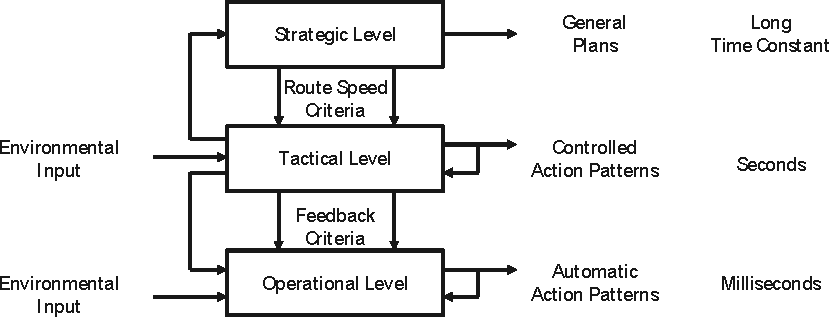
\includegraphics[width=\textwidth]{images/tele_operated_driving/5gaa_tod_use_cases_and_requirements_fig1.pdf}
    \caption{The hierarchical structure of driving tasks, from \cite{5gaa_tod_use_cases_and_requirements}}
    \label{fig:5gaa_tod_use_cases_and_requirements}
\end{figure}

The 5GAA also defines four levels for the involvement of the Tele-Operated Driving operator with the act of driving, ranging from none to total:

\begin{itemize}
    \item \textit{Non-ToD}: the ToD operator takes no role in the act of driving and all levels mentioned above are performed by the in-vehicle driver, be it human or not.
    \item \textit{Dispatch ToD}: the ToD operator acts as the Dispatcher, which performs the Strategic Level operations of driving, while the Tactical and Operational level operations are performed by the in-vehicle user.
    \item \textit{Indirect Control ToD}: the ToD operator acts as the Indirect Controller, or Remote Assistant, which performs the Tactical Level operations and, if needed, the Strategic Level operations.
    \item \textit{Direct Control ToD}: the ToD operator acts as the Direct Controller, or Remote Driver, which performs all or part of the real-time Operational Level functions. If needed, the operator may also perform Tactical and Strategic level operations.
\end{itemize}

Table~\ref{tab:5gaa_tod_role_and_engagement} summarizes the distinction between ToD types with respect to the driving activity levels.


\begin{table}[H]
\begin{tabular}{|c|ccc|}
\hline
 &
  \multicolumn{3}{c|}{\textbf{Driving Activity}} \\ \cline{2-4} 
\multirow{-2}{*}{\textbf{ToD Type}} &
  \textbf{\begin{tabular}[c]{@{}c@{}}Strategic\\ Operation\end{tabular}} &
  \textbf{\begin{tabular}[c]{@{}c@{}}Tactical\\ Operation\end{tabular}} &
  \textbf{\begin{tabular}[c]{@{}c@{}}Operational level\\ Operation\end{tabular}} \\ \hline
\textbf{Non-ToD} &
  \begin{tabular}[c]{@{}c@{}}In-Vehicle user\\ or system\end{tabular} &
  \begin{tabular}[c]{@{}c@{}}In-Vehicle user\\ or system\end{tabular} &
  \begin{tabular}[c]{@{}c@{}}In-Vehicle user\\ or system\end{tabular} \\ \cline{2-2}
\textbf{Dispatch ToD} &
  \multicolumn{1}{c|}{\cellcolor[HTML]{67FD9A}ToD operator} &
  \begin{tabular}[c]{@{}c@{}}In-Vehicle user\\ or system\end{tabular} &
  \begin{tabular}[c]{@{}c@{}}In-Vehicle user\\ or system\end{tabular} \\ \cline{3-3}
\textbf{Indirect Control ToD} &
  \cellcolor[HTML]{9AFF99}\begin{tabular}[c]{@{}c@{}}ToD operator\\ (if needed)\end{tabular} &
  \multicolumn{1}{c|}{\cellcolor[HTML]{67FD9A}ToD operator} &
  \begin{tabular}[c]{@{}c@{}}In-Vehicle user\\ or system\end{tabular} \\ \cline{4-4} 
\textbf{Direct Control ToD} &
  \cellcolor[HTML]{9AFF99}\begin{tabular}[c]{@{}c@{}}ToD operator\\ (if needed)\end{tabular} &
  \cellcolor[HTML]{9AFF99}\begin{tabular}[c]{@{}c@{}}ToD operator\\ (if needed)\end{tabular} &
  \cellcolor[HTML]{67FD9A}{\color[HTML]{FE0000} ToD operator} \\ \hline
\end{tabular}
\caption{Tod Operator engagement in the act of driving in different types of ToD, adapted from \cite{5gaa_tod_use_cases_and_requirements}}
\label{tab:5gaa_tod_role_and_engagement}
\end{table}

The focus of this thesis' performance evaluation will be the simulation of a Direct-Control ToD service, with operational level operation.

\section{Use cases}
The variety of applicable use cases for Tele-Operated Driving is endless. This section will introduce some of them.

The main use case, as defined by the 5GCroCo project \cite{5gcroco} and depicted in \figurename~\ref{fig:5gcroco_obstacle_avoidance}, involves the event of a ToD operator taking direct control of an otherwise-autonomous vehicle in the case of an unexpected road blockage or difficult section that it cannot handle by itself.
The vehicle comes to a safe stop and control is handed over to the remote operator, which from their virtual cockpit connects to the video and sensor feed and provides the required controls to overcome the difficult situation. After the obstacle is avoided, the operator brings the vehicle to a stop once again and the Autonomous Driving function takes over and continues on its task.

The 5GAA \cite{5gaa_tod_system_requirements_architecture} lists several more use cases, including:
\begin{itemize}
    \item Remote driving in the context of a car-sharing service for a trip from airport to city center.
    \item Tele-operated Driving for automated parking.
    \item Remote driving for vehicles in situations where human access is not possible or too dangerous.
\end{itemize}

\begin{figure}[H]
    \centering
    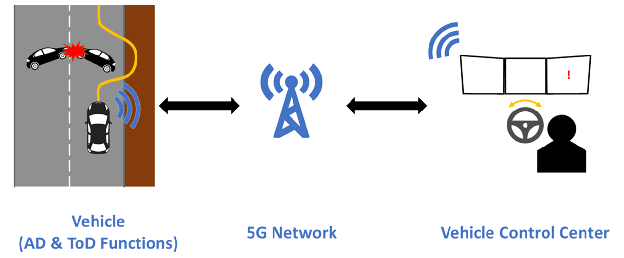
\includegraphics[width=\textwidth]{images/tele_operated_driving/5gcroco_obstacle_avoidance}
    \caption{Remotely controlled maneuvering around a road blockage, from \cite{5gcroco}}
    \label{fig:5gcroco_obstacle_avoidance}
\end{figure}

\section{Functional requirements}
In \cite{5gaa_tod_use_cases_and_requirements} and \cite{5gaa_tod_system_requirements_architecture} a series of functional requirements are described for the host vehicle, the ToD operator, the communication network and the infrastructure. This thesis will focus on the first three categories and requirements relevant to Direct-Control ToD.

\subsection{Host Vehicle requirements}
The Host Vehicle must meet the following functional requirements in order to engage in Tele-Operated Driving:
\begin{itemize}
    \item The vehicle should keep track of its geographical position and report it to the ToD Service Provider when required.
    \item The vehicle should be able to verify and calibrate its perception sensors and ensure they are in a proper state for engaging in the ToD service.
    \item The vehicle should be able to detect any malfunctioning of the ToD system and override the controls in order to bring itself to a minimal risk condition, e.g.\ pull over safely to the side of the road. For example, in the case of a loss of connectivity, a physical intrusion in the vehicle, or any other fault leading to incorrect actuation data.
    \item The vehicle should share sensor information with the ToD operator, which includes video streams, LiDAR, and RADAR data, when required.
    \item If regulations require it, the vehicle should be able to store communication relevant to the ToD service for later evaluation, inspection and analysis.
    \item The vehicle should be able to report the operations and status of the ToD service to the in-vehicle system or user, e.g.\ whether the ToD operator is currently engaged in the service.
    \item The vehicle sub-system should take steps to protect the ToD service from security threats and malicious actors trying to gain control of the vehicle's movement.
    \item The vehicle should be able to process the remote actuator commands.
    \item The vehicle should receive maneuver instructions from the ToD operator and execute them, according to its internal security checks.
\end{itemize}

\subsection{ToD operator requirements}
The ToD operator subsystem must be able to fulfill the following requirements in order to allow for safe operation:
\begin{itemize}
    \item The ToD operator should be able to acquire all ToD-related parameters of the vehicle in a real-time manner, e.g.\ ToD type, vehicle capability, and sensor data.
    \item The ToD operator should be able to detect the malfunctioning of a ToD system and bring the vehicle to a minimal risk condition.
    \item The ToD operator should be able to disengage the ToD function in a safe manner at the end of its tasks.
    \item The ToD operator subsystem should be able to obtain sensor data and information from the vehicle, weather conditions, and infrastructure data, and display it to the ToD operator to enhance the remote driving experience.
    \item The ToD operator subsystem should be able to authenticate and authorize the human ToD operator and machine ToD apps/entities.
    \item The ToD operator should be able to send commands to the vehicle for the purpose of remote control.
    \item The ToD operator should be able to change the ToD type when required.
    \item The ToD operator should be able to monitor the network parameters and be swiftly informed about changes in its performance.
    \item The ToD operator should be able to monitor the latency and quality of the video signal at all times.
    \item The ToD operator sub-system should be able to display real-time video around the vehicle to the operator with acceptable quality in order to provide a good user experience.
\end{itemize}

\subsection{Communication network requirements}
The communication network is essential for allowing data exchange between HV and ToD operator. In particular, the following criteria must be met:
\begin{itemize}
    \item The communication network should provide the ability for the ToD operator to establish a mutually authenticated and secure communication session with the vehicle.
    \item The communication network should guarantee service continuity during the operation of the ToD service.
    \item The communication link should be reliable and encrypted.
    \item The communication session should be kept active even when roaming different networks and across national borders. The ToD operator and vehicle should be informed in advance in case this is not possible.
    \item The communication network should be able to notify the vehicle and the ToD operator about sudden changes in network conditions.
    \item The communication network should inform the vehicle and the ToD operator about its measured latency information.
\end{itemize}

\section{Technical requirements}
Other than functional requirements, it is important to establish some technical requirements in order to obtain a reliable and safe operation.

\subsection{Latency}
The 5GAA defines service level latency as: ``\textit{measurements of time from the occurrence of the event in scenario application zone to the beginning of the resulting actuation}''~\cite{5gaa_tod_system_requirements_architecture}.
Network latency, while being the most crucial aspect and the one subject to the most variability, as it will be shown later, only comprises a part of the chain of delay-inducing processes, which include on the uplink (Vehicle to Operator):
\begin{itemize}
    \item The elapsed time between an event happening in the world and the sensors acquiring the raw data.
    \item The elapsed time between the sensors capturing the event and them transmitting the data to the vehicle's communication unit, which takes some time to process it.
    \item The network latency in relaying the transmitted information to the ToD operator's location, including the mobile network and backend systems.
    \item The latency induced by the ToD Operator App to decode, process and present the received information
    \item The time the ToD operator needs to perceive and react to the presented information.
\end{itemize}
Correspondingly, on the downlink (Operator to Vehicle):
\begin{itemize}
    \item The time the ToD operator (if human) takes to move the controls.
    \item The elapsed time between the controls being moved and the movement getting registered by the sensors.
    \item The elapsed time between the movement being captured and it being processed and stored into a packet to be transmitted back to the vehicle.
    \item The communication latency induced by the network from the ToD operator's location to the vehicle, through backend systems and the mobile network.
    \item The time the vehicle's systems take to decode the data and send the appropriate instructions to the onboard actuators.
    \item The elapsed time between the actuators executing the required action and the vehicle's motion occurring as a result.
\end{itemize}
In the case of video transmission, the delay that occurs between photons of visible light hitting the lens of a camera and the event being portrayed on a display after encoding, transmission, processing and decoding is called \textit{Glass-to-Glass (GTG) delay}. Bachhuber and Steinbach \cite{gtg_delay} have proposed a system that accurately measures GTG delay and provides an image representation of the steps that influence the time an event takes from when it happens to when it's reproduced on the user's display, \figurename~\ref{fig:gtg_delay_measurement_principle}.
\begin{figure}[h]
    \centering
    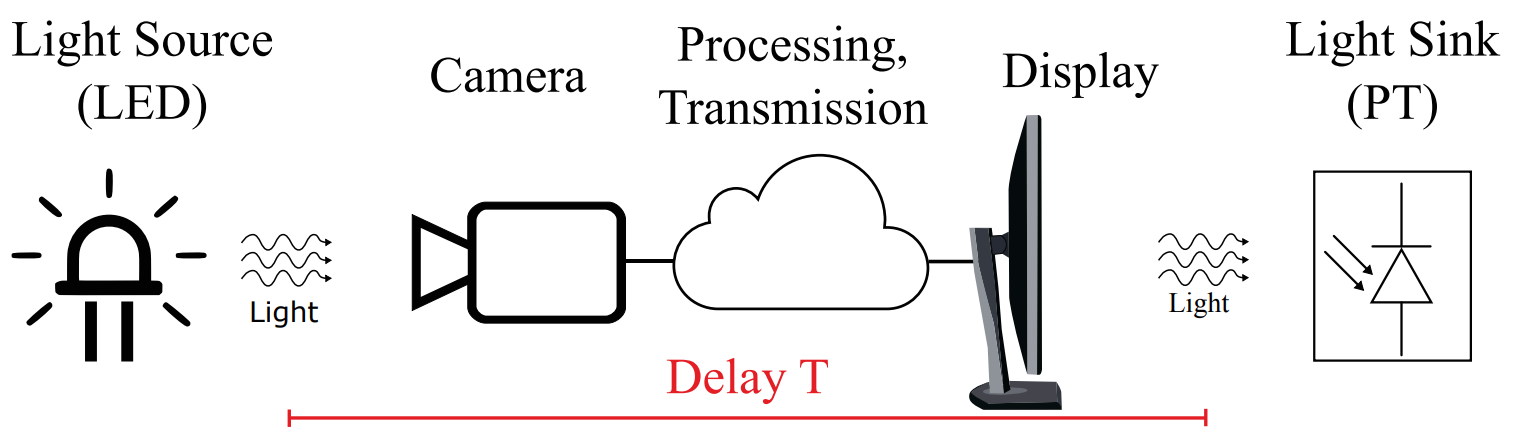
\includegraphics[width=\textwidth]{images/tele_operated_driving/gtg_delay_measurement_principle}
    \caption{GTG delay measurement principle, from \cite{gtg_delay}}
    \label{fig:gtg_delay_measurement_principle}
\end{figure}

% \noindent Correspondingly, on the downlink, the steps that induce a delay are:
% \begin{itemize}
%     \item The sampling latency for input devices to capture the ToD operator's commands.
%     \item The latency for the ToD operator app to collect the input, process it and prepare the data packets it needs to send back to the vehicle.
%     \item The communication latency induced by the network from the ToD operator's location to the vehicle, through backend systems and the mobile network.
%     \item The latency for the app on the Host Vehicle to process and authenticate the data packets containing the commands issued by the operator.
%     \item The latency for the vehicle's onboard actuators to execute the decoded maneuver.
% \end{itemize}
A consideration can be made about the variability of each delay: All but the network and the ToD operator's (in the case of a human) contributions can basically be regarded as fixed values, and once properly tuned and in the absence of faults are not to be concerned about. It is very important then to keep network delay in check as it can make or break the service.

The 5GAA \cite{5gaa_tod_system_requirements_architecture} defines a requirement for the maximum total latency from HV to Operator of 100ms and from Operator to HV of 20ms for a ToD use case up to 50km/h (where the HV will move 0.27m within 20ms).

In a study carried out by Neumeier et al. \cite{teleoperation_latency_matters}, tests indicated that a latency of around 300ms led to a deteriorated driving experience for the candidates, and found a link between added latency and the detriment of the driver's confidence. They also showed that the tolerable latency is severely affected by the environment.

The sensitivity to latency of the service is mostly determined by the difficulty level of the environment around the vehicle and the speed it is traveling at: a low-speed scenario on a straight section of road will be less impacted by a latency spike than a high-speed highway section in the presence of other vehicles and on a curve.


\subsection{Sensors}
In order to allow for the operation of ToD services, the host vehicle must equip a vast array of sensors and fulfill the technical requirements for automated driving according to SAE levels 3, 4, and 5. The 5GAA provides a list of the most relevant ones \cite{5gaa_tod_system_requirements_architecture}.

\subsubsection{HD Digital maps}
High-Definition digital maps act as a sensor by themselves by providing details about the environment, possibly also about real-time conditions. They allow to `see' around curves or in fog.
HD maps support sensor data and show much more than just roads and routes. They capture the three-dimensional environment at a centimeter-accurate resolution and can be compared to the data provided by the onboard sensors from the host vehicle.
Information captured by HD maps may include lane models, traffic signs, road infrastructure, and lane geometry. As the automation level increases, so does the requirement for resolution of these maps.

\subsubsection{Precise positioning}
Precise positioning refers to a series of techniques for correcting GNSS errors in order to provide even higher level of position accuracy in the vehicles, ideally with as small an error as a few centimeters.
Automated driving and ToD operations require at least lane-level precision with very high integrity. This is especially crucial when bad weather conditions, such as heavy snow, impair the other sensors' performance.

\subsubsection{LiDAR capabilities}
LiDAR - Light Detection and Ranging, is a sensor technology used to actively monitor the environment and perceive short-term changes, creating a 3D map of the host vehicle's surroundings. It can operate even under difficult conditions, e.g.\ in darkness, between 50 and 500m, and scan angles up to 180 degrees.

\subsubsection{RADAR capabilities}
RADAR technology is very well known and like LiDAR, it is also used to actively monitor the environment. It's however limited to around 250m and has a narrower scanning angle. On the other hand, RADAR systems are very effective over short distances, starting at 0.2m, and have low processing demands for detecting a wide variety of environmental values, e.g.\ angle, distance, speed, and material parameters.

\subsubsection{Ultrasonic capabilities}
Ultrasonic technology is used to actively monitor the near-field environment of the vehicle, under 1m. It's useful for avoiding collisions while parking or navigating tight spaces.

\subsubsection{Video camera capabilities}
In addition to the aforementioned sensors, it is important that the Host Vehicle also provide a video stream of its surroundings. This is crucial in the case of a human ToD operator but it is useful in the case of a machine operator that might be able to acquire some new information using computer vision that the sensors might not have yet captured.
Cameras are most effective in clear and well-lit conditions, as they are rendered almost useless in heavy fog or dark environments.
Video cameras can additionally be installed on the infrastructure, such as RSUs, lamp posts and traffic masts, in order to provide additional data from a different point of view.

\subsubsection{Microphone and loudspeakers}
Microphones and loudspeakers are useful to monitor and interact with the environment through audio. They can be used to communicate with a passenger, detect relevant outside communication and pick up instructions e.g.\ from police commands or emergency vehicle sirens.

